\section{Theory}

The purpose of this experiment is to see how an interferometer works. The
Michelson interferometer is the design that will be used for the experiment. A
Michelson interferometer is a simple interferometer that is used to make very
small and precise measurements, in fact the Michelson interferometer is the
layout used in LIGO\@. A Michelson interferometer works by having a laser shoot
down a path into a beam splitter that splits the laser beam into two seperate
paths. At the end of each path there is a mirror that will reflect the laser
back toward the beam splitter which then combines the two beams. After the
recombination the lasers will be either in or out of phase, due to the
superposition principle. The superposition principle basically says that when
two waves pass through the same point in space their amplitudes will combine;
this causes the net amplitude to add or subtract, known as constructive and
destructive interference respectively. Constructive interference happens if the
waves are in phase while destructive interference happens when the waves are out
of phase.

\begin{figure}[ht!]
\centering
%Caption: Two waves in phase and the next is two waves 180 degress out of phase
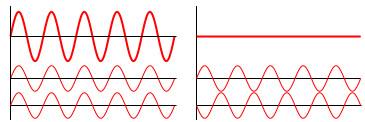
\includegraphics[width=4 in]{Interference_of_two_waves.png}
\end{figure}

In this experiment the only way that the phase will change will be due to the distance between the mirrors and the beam splitter. The phase difference,$\Delta \phi$, is calculated by 
	\begin{align}
		\nonumber \Delta \phi &=\frac{2\pi}{\lambda} \Delta p
	\end{align}
with $\Delta p$ being the difference in the paths and $\lambda$ being the wavelength of the laser being used. From there we can then say that 
	\begin{align}
		\nonumber \Delta p &=\sum(n_2 d_2)-\sum(n_1 d_1) \\
		\nonumber		&=n_2 d_2 - n_1 d_1
	\end{align} 
where $d$ is the distance from the beam splitter to the cube and $n$ is index of refraction of the medium the beam is traveling through. For this experiment the medium's are the same, they are both traveling through air, so then $n_1=n_2$ which results in
	\begin{align}
		\nonumber \Delta p &= n_2 d_2 - n_1 d_1 \\
		\nonumber 	&= n(d_2 - d_1) \\
		\nonumber \Delta \phi &=\frac{2\pi n}{\lambda} (d_2 - d_1)
	\end{align}

The change in phase will then affect the intensity of the beam, causing fringes to appear. These fringes will be red and black rings on a screen or piece of paper behind the lens. The black rings signify a destructive interference while the red rings are due to the constructive interference. 

Using a photodiode to get the fringes to appear on an oscilloscope it is then possible to get the voltage required to move from one fringe to another. Using this information with the properties of the piezo stack it is possible to get the wavelength of the laser. 


